\documentclass[red]{tutorial}



\usepackage[no-math]{fontspec}
\usepackage{xpatch}
	\renewcommand{\ttdefault}{ul9}
	\xpatchcmd{\ttfamily}{\selectfont}{\fontencoding{T1}\selectfont}{}{}
	\DeclareTextCommand{\nobreakspace}{T1}{\leavevmode\nobreak\ }
\usepackage{polyglossia} % English please
	\setdefaultlanguage[variant=us]{english}
%\usepackage[charter,cal=cmcal]{mathdesign} %different font
%\usepackage{avant}
\usepackage{microtype} % Less badboxes



\usepackage[charter,cal=cmcal]{mathdesign} %different font
%\usepackage{euler}
 
\usepackage{blindtext}
\usepackage{calc, ifthen, xparse, xspace}
\usepackage{makeidx}
\usepackage[hidelinks, urlcolor=blue]{hyperref}   % Internal hyperlinks
\usepackage{mathtools} % replaces amsmath



\usepackage{bbm} %lower case blackboard font
\usepackage{amsthm, bm}
\usepackage{thmtools} % be able to repeat a theorem
\usepackage{thm-restate}
\usepackage{graphicx}
\usepackage{xcolor}
\usepackage{multicol}
\usepackage{fnpct} % fancy footnote spacing

 
\newcommand{\xh}{{{\mathbf e}_1}}
\newcommand{\yh}{{{\mathbf e}_2}}
\newcommand{\zh}{{{\mathbf e}_3}}
\newcommand{\R}{\mathbb{R}}
\newcommand{\Z}{\mathbb{Z}}
\newcommand{\N}{\mathbb{N}}
\newcommand{\Perp}{\mathrm{perp}}
\newcommand{\Span}{\mathrm{span}\,}
\newcommand{\Img}{\mathrm{img}\,}
\newcommand{\Null}{\mathrm{null}\,}
\newcommand{\Range}{\mathrm{range}\,}
\newcommand{\rref}{\mathrm{rref}}
\newcommand{\Rank}{\mathrm{rank}}
\newcommand{\nnul}{\mathrm{nullity}}
\newcommand{\mat}[1]{\begin{bmatrix}#1\end{bmatrix}}
\newcommand{\chr}{\mathrm{char}}
\renewcommand{\d}{\mathrm{d}}


\theoremstyle{definition}
\newtheorem{example}{Example}[section]
\newtheorem{defn}{Definition}[section]

%\theoremstyle{theorem}
\newtheorem{thm}{Theorem}[section]

\pgfkeys{/tutorial,
	name={Tutorial 3},
	author={Jason Siefken \& Bernardo Galv\~ao-Sousa},
	course={MAT 244},
	date={},
	term={},
	title={Modelling with Parametres}
	}

\begin{document}
	\begin{tutorial}
				\begin{objectives}
	In this tutorial you will explore orthogonality in depth.

	These problems relate to the following course learning objectives:
	\textit{Work independently to understand concepts and procedures that have not been previously
		explained to you},
		\textit{translate between algebraic and geometric viewpoints to solve problems}, and
		\textit{understand definitions that have been written by others}.
		\end{objectives}

		\vspace{-.4cm}
\subsection*{Definitions}
		Recall the vectors $\vec a$ and $\vec b$ are \emph{orthogonal} if $\vec a\cdot \vec b=0$.
		We say the \emph{sets $A$ and $B$ are orthogonal} if every vector in $A$ is orthogonal to every
		vector in $B$.

		\vspace{-.4cm}
\subsection*{Problems}
Let $\vec v_1=\mat{1\\1\\1\\1}$,
		$\vec v_2=\mat{-1\\1\\1\\1}$,
		$\vec v_3=\mat{-1\\-1\\1\\1}$,
		$\vec v_4=\mat{1\\0\\0\\1}$,
		$\vec v_5=\mat{3\\-1\\-1\\-1}$, and
		$\vec v_6=\mat{1\\1\\2\\0}$.

\begin{enumerate}
	\item
	\begin{enumerate}
		\item Identify all pairs of orthogonal vectors among $\vec v_1$, \ldots, $\vec v_6$.
		\item Let $A=\{\vec v_1, \vec v_2\}$ and $B=\{\vec v_3,\vec v_4\}$. Are $A$ and $B$ orthogonal sets?
			Why or why not?
		\item Let $P=\{\vec v_1, \vec v_6\}$ and $Q=\{\vec v_3,\vec v_5\}$. Are $P$ and $Q$ orthogonal sets?
			Why or why not?
		\item Can you split the vectors $\vec v_1$, \ldots, $\vec v_6$ into two non-empty sets that are orthogonal to
			each other? Explain.
	\end{enumerate}
	\item
	\begin{enumerate}
		\item Using guess-and-check, find two vectors that are orthogonal to both $\vec v_1$ and $\vec v_2$.
		\item Set up and solve a system of equations to find all vectors orthogonal to $\vec v_1$ and $\vec v_2$.
	\end{enumerate}
	\item The dot product is \emph{commutative} and \emph{distributive}. That is $\vec v\cdot (\alpha\vec a+\vec b)=
		(\alpha\vec a+\vec b)\cdot \vec v=\alpha(\vec a\cdot \vec v)+\vec b\cdot\vec v$. Use this to show that if
		the set $X=\{\vec x\}$ is orthogonal to the set $Y=\{\vec y_1,\vec y_2,\vec y_3,\vec y_4\}$,
		then $X$ is also orthogonal to $\Span Y$.
	
	\item We say that $\vec a$ and $\vec b$ are \emph{close} if $\|\vec a-\vec b\|$ is small. We will see if we can
		extend this concept to lines.

		Let the lines $\ell_1$, $\ell_2$, $\ell_3$, and $\ell_4$ be given by the equations $y=x$, $y=1.001x$,
				$y=2000x$, $y=3000x$.
		\begin{enumerate}
			\item Out of $\ell_1$, \ldots, $\ell_4$, which lines would you call ``close''? Can you come up
				with a mathematical definition to justify your conclusion?
			\item For $\ell_1$, \ldots, $\ell_4$, find unit normal vectors $\vec n_1$, \ldots, $\vec n_4$.
				For consistency, ensure each unit normal vector points towards the upper left (i.e., has negative first coordinate
				and positive second coordinate).
			\item Compute the distances between $\vec n_1$, \ldots, $\vec n_4$. Do these distances coincide with your
				intuition about closeness? Why might comparing normal vectors be preferable to comparing direction vectors?
		\end{enumerate}
	
\end{enumerate}
	\end{tutorial}

	\begin{solutions}
				\begin{enumerate}
			\item \begin{enumerate}
				\item \phantom{x}
				
				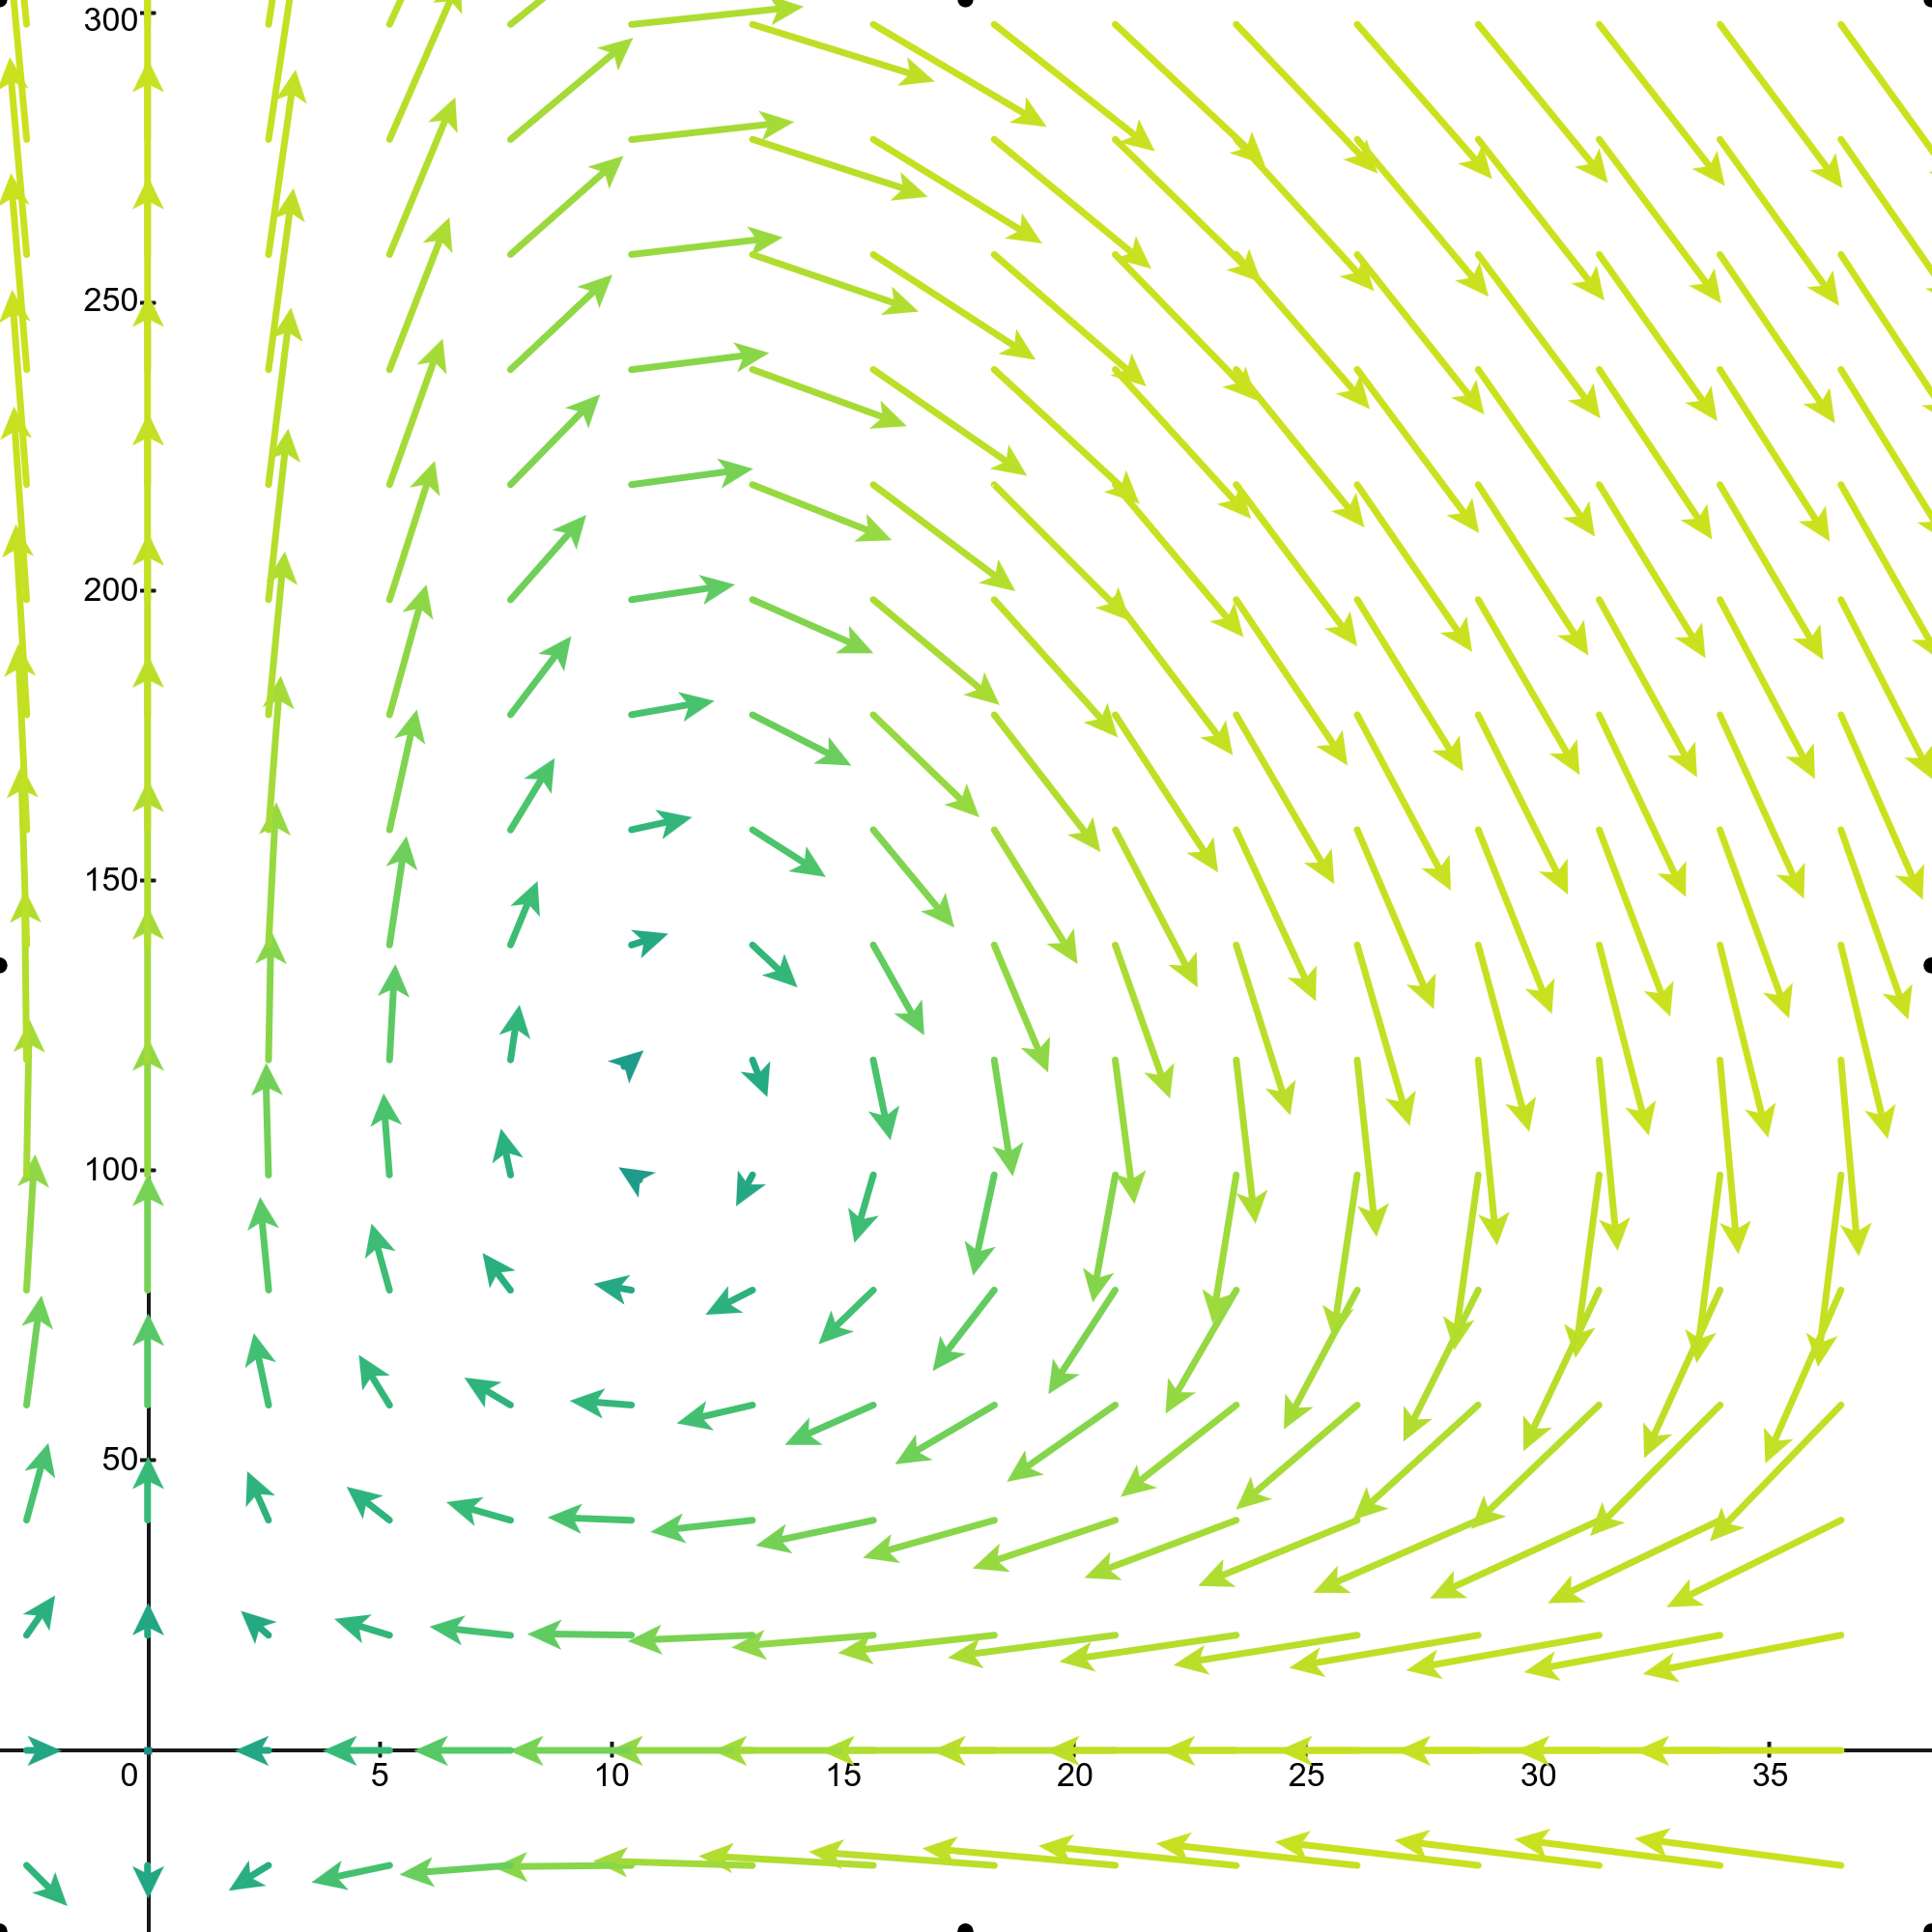
\includegraphics[width=3in]{resources/tutorial-02-1a.png}

				\item Arrows to the right of $F=11$ point down. That means as there are more foxes, the rabbit population decreases.
				Arrows to the left of $F=11$ point up, so as there are fewer foxes, there are more rabbits. If the arrows were oriented in the opposite direction,
				more foxes would lead to more rabbits, which is the opposite of what we would expect if the foxes ate the rabbits.
			\end{enumerate}
			\item \begin{enumerate}
				\item As long as $a,b,c,d>0$, there will be periodic behaviour.
				However, if any of the parameters becomes zero, the behaviour will change.
				\item 
				\item If we leave $a,c,d$ as they are and set $b$ to zero, the foxes will never die.
				Thus, the fox population will grow and grow as long as there are rabbits available. However,
				once the foxes eat the rabbits to extinction, they fox population will be unchanged, since the foxes are
				immortal!
			\end{enumerate}
			\item \begin{enumerate}
				\item We know that a maximum rabbit population occurs when $R'=0$. Manipulating the equation for
				$R'$, we find that $R'=0$ when $F=c/d$.
				\item Manipulating the equation for $F'$, we find that $F'=0$ when $R=b/a$.
				\item If neither populations change, then we must have $F'=0$ and $R'=0$. This occurs when
				$(F,R)=(c/d, b/a)$ or $(F,R)=(0,0)$.
				\item If we allow $d$ or $a$ to be zero, the derivations we did in the previous parts
				are no longer valid (we can't divide by zero)! If $c$ or $d$ equals zero, then there are equilibrium solutions
				where one population is positive and the other zero. Since populations cannot be negative, this prevents
				periodic behaviour. So, our analysis here helps explain part \ref{qual}.
			\end{enumerate}
		\end{enumerate}

	
	\end{solutions}
	\begin{instructions}
		\subsection*{Learning Objectives}
	Students need to be able to\ldots
	\begin{itemize}
		\item Switch between phase portraits and component graphs.
		\item Recognize the difference between solutions and curves in phase space.
		\item Deduce properties of equilibrium solutions from phase portraits.
	\end{itemize}

\subsection*{Context}
	We have analyzed systems of ODEs in class and in tutorial using phase portraits. We are getting ready to
	study systems of ODEs and equilibrium solutions to system written in matrix form. This requires a very good
	understanding of phase portraits and how they relate to solutions to systems.

\subsection*{What to Do}
	Introduce the learning objectives for the day's tutorial. Explain that phase portraits/graphs in phase space are an important
	tool in the study of differential equations and we want to better understand how graphs in phase space
	relate to solutions to systems of ODEs.

	Start by asking students to recall what we mean when we say ``phase portrait'' and ``component space'' for a system of ODEs
	$A'(t)=\ldots$ and $B'(t)=\ldots$. \emph{Do not give a lecture on this}, but you may have a short discussion ($< 5$ min)
	on this distinction.
	
	After most groups have finished \#1, go over it as a class. Doing so will ensure everyone has a baseline understanding
	of the distinction between phase space and component space.

	Continue as usual, walking around the room and asking
		questions while letting students work on the next problem and gathering them together
		for discussion when most groups have finished.

		7 minutes before class ends, pick a suitable problem to do as a wrap-up. Most likely, \#3 will be a good choice.



	
\subsection*{Notes}
	\begin{enumerate}
		\item Hopefully this problem won't be hard for them. All the vertices line up, after all. If they are struggling,
		it is worth spending a lot of time on this question, since they cannot use phase portraits unless they understand this.

		\item Students will struggle getting a curve for this question. If they are struggling, have them approximate
		the curve with a polygon and try to find component graphs for the polygon first. Then they can ``smooth it out''
		to get the curve.
		
		Part (b) will be especially hard. Some will struggle to even understand what the question is asking.

		\item This question is a good wrap-up question. It should be quicker than all the other questions.

		\item This is a question for groups who have moved more quickly. Students may have forgotten what an equilibrium
		solution is. Ask them to check their notes for the definition.

		Part (c) introduces a brand new definition. Assure students that they have not learned this definition in class
		and that's okay!

	\end{enumerate}
	\end{instructions}

\end{document}
